\chapter{Received Signal Simulations} \label{ch:simulations}
%define the signal characteristics and evaluate the properties of the resulting signal over the parameter sweeps

\section{Introduction}
The following simulations performed will define the search space on the effect of rotor blade modulation. Since the software developed allows for full parameterization of the objects within the scene, the simulations will focus on a few that effect the different object's positions in 3D space and the resulting received signal. The parameters that will be changed are the position of the receiver, pitch of the rotor blade, and transmitter position. The effect of each parameter will be analyzed to determine what information can be derived for localization.

%-----------------------------------------------------------------------------------------------------------------------------------------------------------------------

\section{Analysis Techniques}
The data from the CSV files generated by the raytracing program are loaded into MATLAB scripts to process the data. The processing technique used is the spectrogram function that computes the short time Fourier transform. This allows for computations to be done in the time frequency domain and provides an accurate picture of how the signal is changing with time. Figure \ref{fig:test_spec} shows an example of the computed spectrograms.

%short Fourier transform alg

\begin{figure}
	\begin{center}
		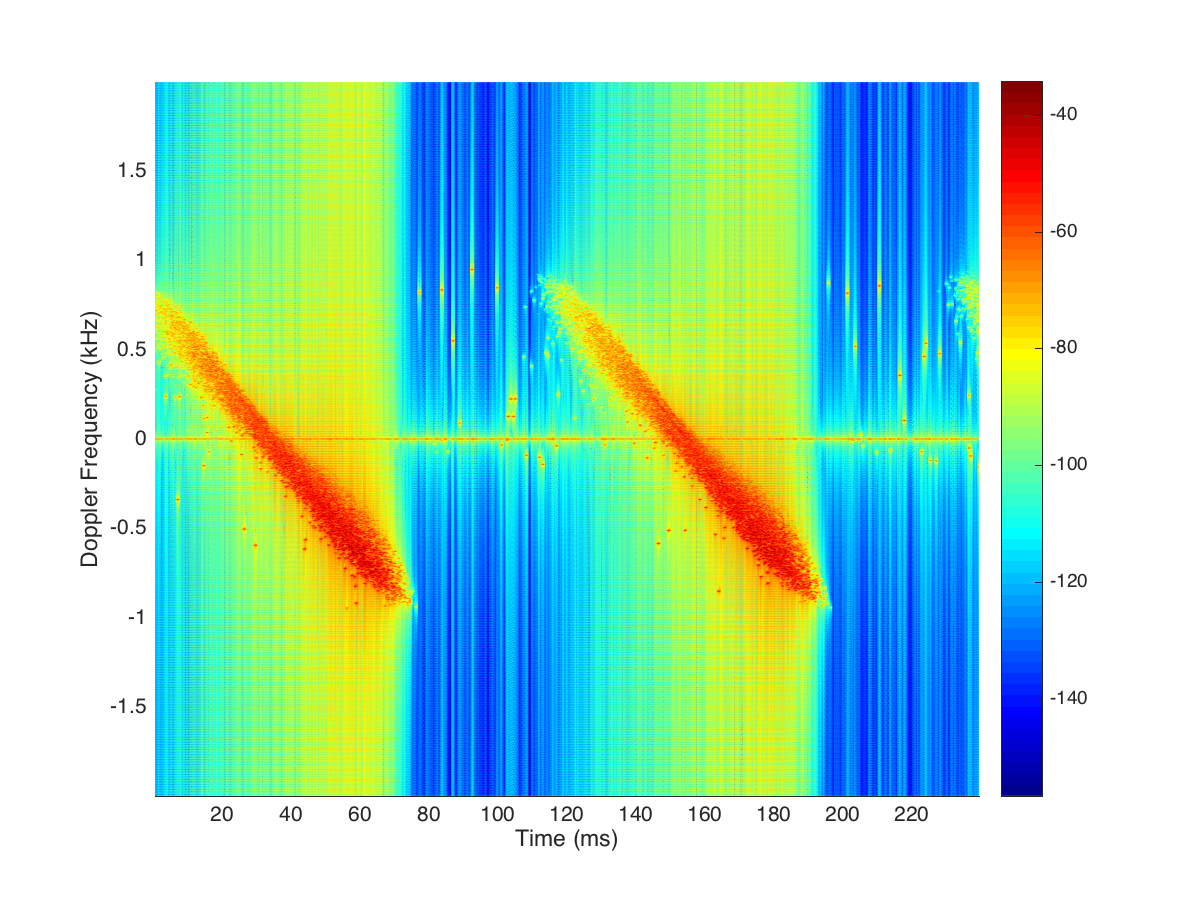
\includegraphics[width=15cm]{images/simulation/test_analysis_spectrogram.eps}
		\caption{Example Spectrum for one Blade revolution with transmitter at Azimuth of 45\textdegree \space and Elevation of 35\textdegree}
		\label{fig:test_spec}
	\end{center}
\end{figure}

After the computation of the short time Fourier transform; the Doppler envelope is calculated by performing a threshold on the power, in both the positive and negative Doppler, at each time slice. The envelope value for that time slice is found by approaching zero frequency and stopping as the power reaches a predetermined level from both the negative and positive values. The power level to set the threshold is calculated differently based on whether the elevation or the azimuth parameter is being swept. For the azimuth angle sweep, which will be shown later in section \ref{taa}, the maximum power is found in each time slice then those values are averaged. Then for each successive angle the same average is taken and averaged with all the others. 

%equation for power averaging over successive angles

This technique is used because the elevation angle is remaining constant, so the distance with the helicopter platform should be constant as well. When varying the elevation angle in section \ref{sec:tea}, the same method cannot be used because the distance is changing so only the maximum power is found in each time slice. Then all those values are averaged without any successive averaging.

\begin{figure}
	\begin{center}
		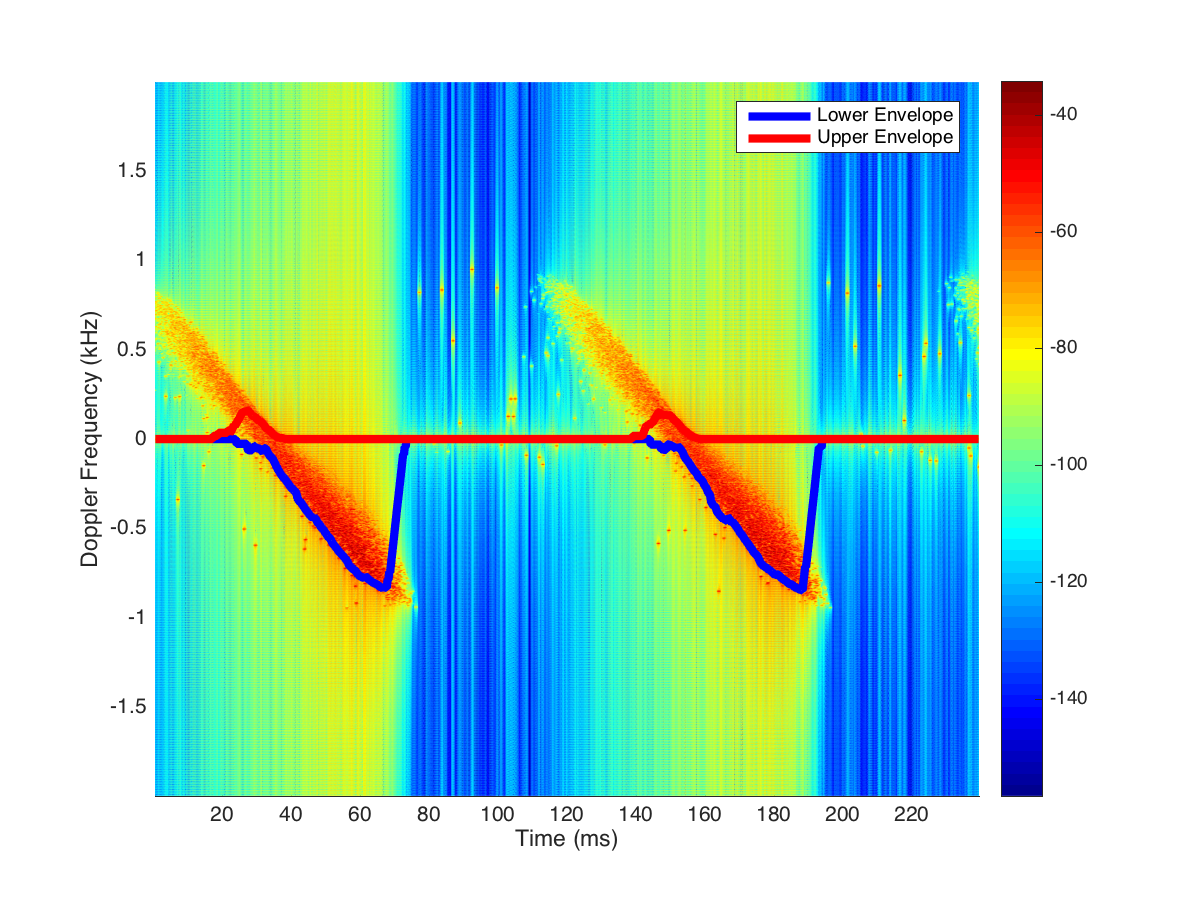
\includegraphics[width=15cm]{images/simulation/test_analysis_spectrogram_with_envelope.eps}
		\caption{Example Spectrum with Doppler Profile for one Blade revolution with transmitter at Azimuth of 45\textdegree \space and Elevation of 35\textdegree}
		\label{fig:test_spec_w_doppler_profile}
	\end{center}
\end{figure}

The Doppler envelopes are displayed in Figure \ref{fig:test_spec_w_doppler_profile}, the lower in blue and the upper in red. The minimum is calculated from the lower envelope, and the maximum from the upper envelope. Those values are then used to characterize that Doppler profile and analyze signal trends as different variables change.

%-----------------------------------------------------------------------------------------------------------------------------------------------------------------------
\section{Receiver Position}
%display spectrograms of the rx position and its affect on doppler and pick a value 7m for all subsequent tests
%use reasoning on cleaner signal more signal variation.
The position of the receiver is determined ultimately by its location on the physical aircraft. The position can be anywhere along the length of the body of the helicopter, but for the purpose of the simulation the receiver position will be varied from directly underneath the rotor to just past the tip. 

%figure of the receiver position 0 to 9m
\begin{figure}
	\begin{center}
		\includegraphics[width=9cm]{images/simulation/rotor_rx_position.eps}
		\caption{Position of the Receiver in Relation to the Rotor Blades}
		\label{fig:rx_position_image}
	\end{center}
\end{figure}

The rotor blade length from Figure \ref{fig:rx_position_image} is 7.5 m so the receiver will be varied from 0 m to 9 m in 1 m increments. The resulting signal is analyzed by calculating its Doppler envelope. Then the maximum and minimum of that envelope will then be used to determined the overall effect of the position of the receiver.

%figure of maximum doppler vs rx position
\begin{figure}
	\begin{center}
		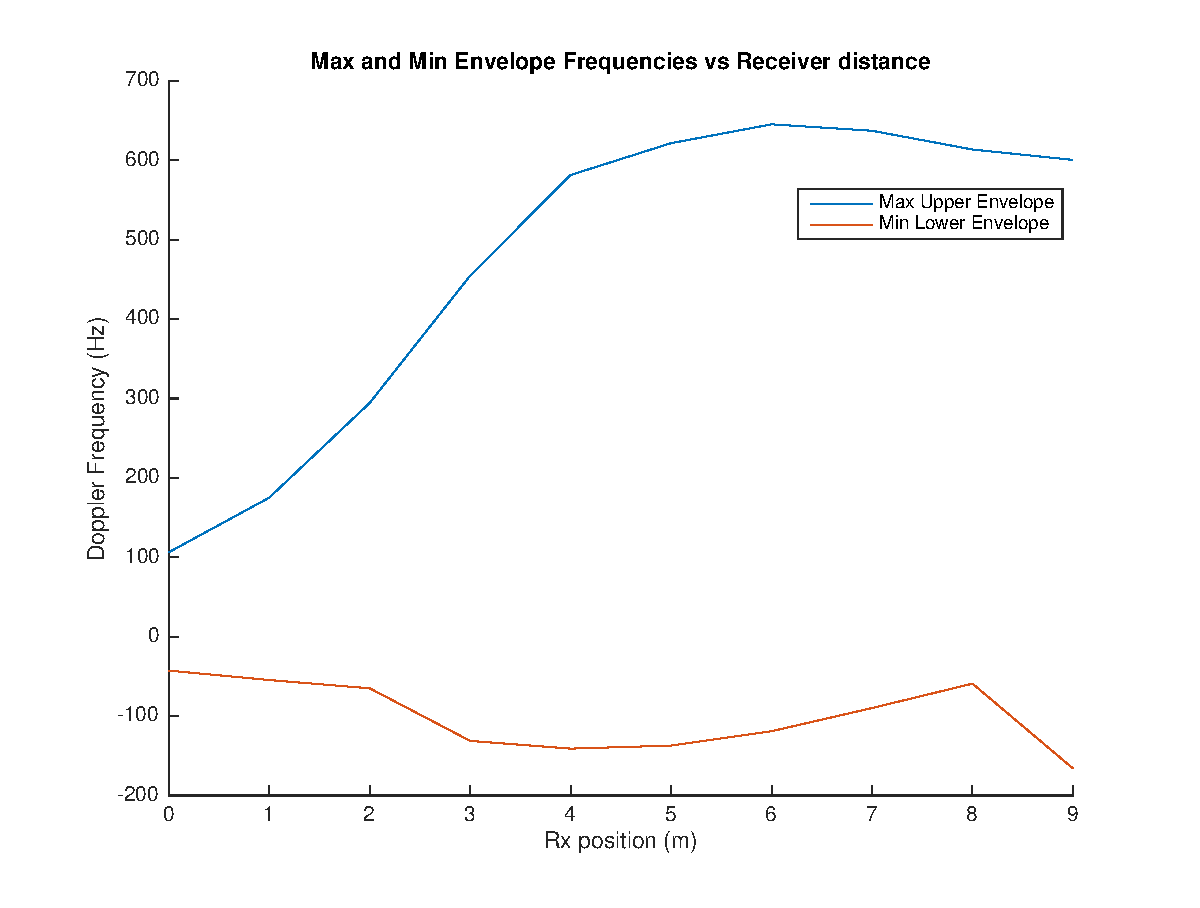
\includegraphics[width=10cm]{images/simulation/receiver_position_max_doppler.eps}
		\caption{Max and Min Doppler vs. Receiver Position with Tx Azimuth at 135\textdegree \space and Elevation at 54\textdegree}
		\label{fig:rx_position}
	\end{center}
\end{figure}
%azimuth = 135, elevation = 54deg

Figure \ref{fig:rx_position} shows maximum Doppler versus the position of the receiver. From this graph, the maximum Doppler frequency changes significantly as the receiver is moved from directly underneath the rotor to past the tip of the rotor at 9 m.The position of the receiver also effects the resulting signal envelope shapes shown in Figures \ref{fig:rx_position_0m} and \ref{fig:rx_position_7m}.

%figure of spectrogram at 0m -- figure of spectrogram at 7m side by side
\begin{figure}
	\begin{center}
		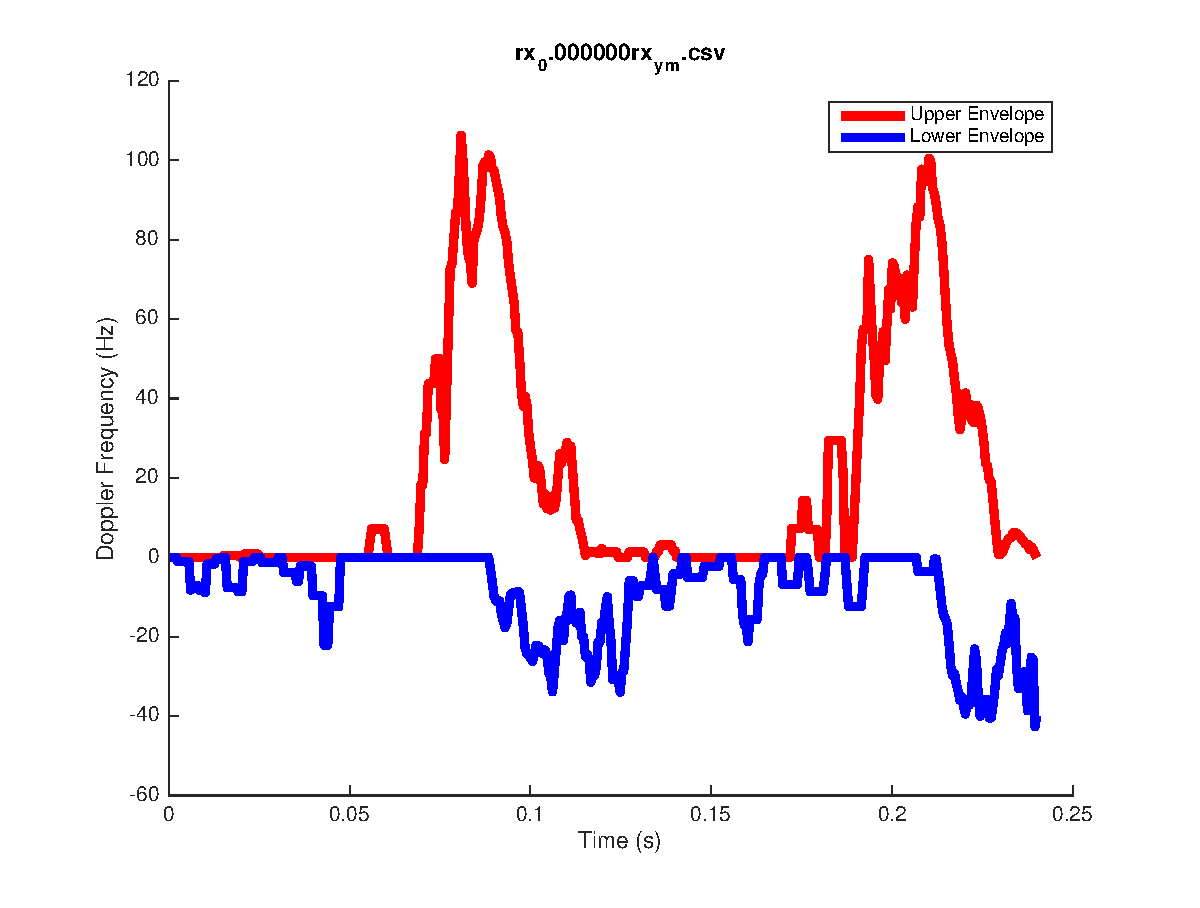
\includegraphics[width=10cm]{images/simulation/Doppler_Receiver_0m.eps}
		\caption{Doppler Envelope with receiver at 0m}
		\label{fig:rx_position_0m}
	\end{center}
\end{figure}

\begin{figure}
	\begin{center}
		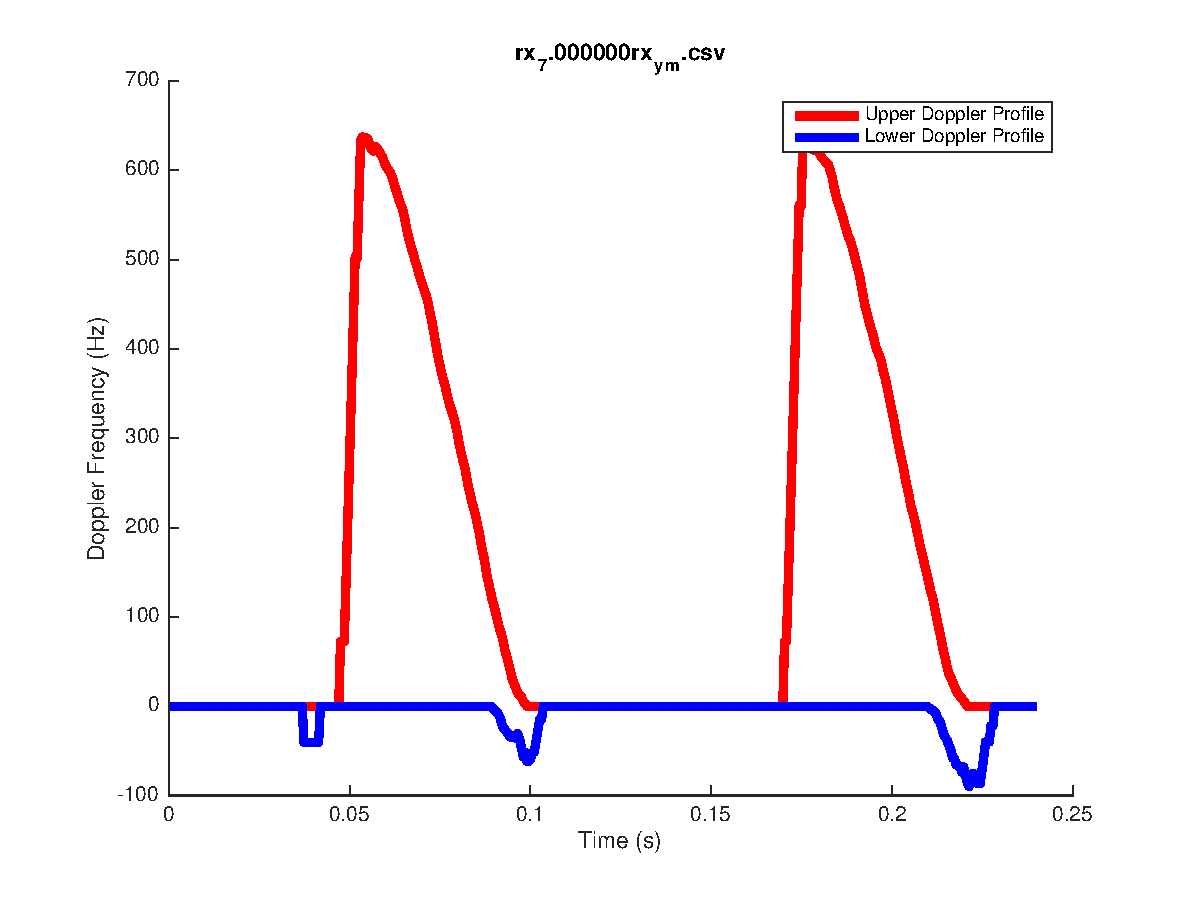
\includegraphics[width=10cm]{images/simulation/Doppler_Receiver_7m.eps}
		\caption{Doppler Envelope with receiver at 7m}
		\label{fig:rx_position_7m}
	\end{center}
\end{figure}

Comparing the received signal envelopes Figure \ref{fig:rx_position_0m} and \ref{fig:rx_position_7m} the maximum Doppler increase reflects the information in Figure \ref{fig:rx_position}. The envelope in Figure \ref{fig:rx_position_0m} is also much noisier than the envelope of Figure \ref{fig:rx_position_7m} and the signal envelope, for the receiver is at 7 m, has a distinctive shape with less variation between its two peaks. The position of the receiver will also determine whether the azimuth angle can be derived from the resulting signal shown later in section \ref{taa}. Therefore, the receiver will be offset from the center of rotation by 7 m for the subsequent simulations.


%-----------------------------------------------------------------------------------------------------------------------------------------------------------------------
\section{Rotor Pitch}
%display spectrograms of rotor pitch from 0 to -15 deg nominal value, then evaluate the effect.
%try to show that pitch does not change the signal significantly
The pitch of the rotor blades determines the amount of lift the rotors create. The pitch range is determined by the shape of the airfoil and the angle at which it will stall and no longer produce lift. For the purpose of the simulations, and the selected airfoil, the pitch range will be from 0\textdegree  \space to 15\textdegree.

%figure of pitched airfoil at 0 and at 15 deg
\begin{figure}
	\begin{center}
		\includegraphics[width=9cm]{images/simulation/pitch.eps}
		\caption{Rotor Pitch}
		\label{fig:blade_pitch}
	\end{center}
\end{figure}

The resulting signal is analyzed by calculating its Doppler envelope. Then the maximum and minimum of that envelope will then be used to determined the overall effect of pitching the rotor blade. 

%figure of doppler vs pitch
\begin{figure}
	\begin{center}
		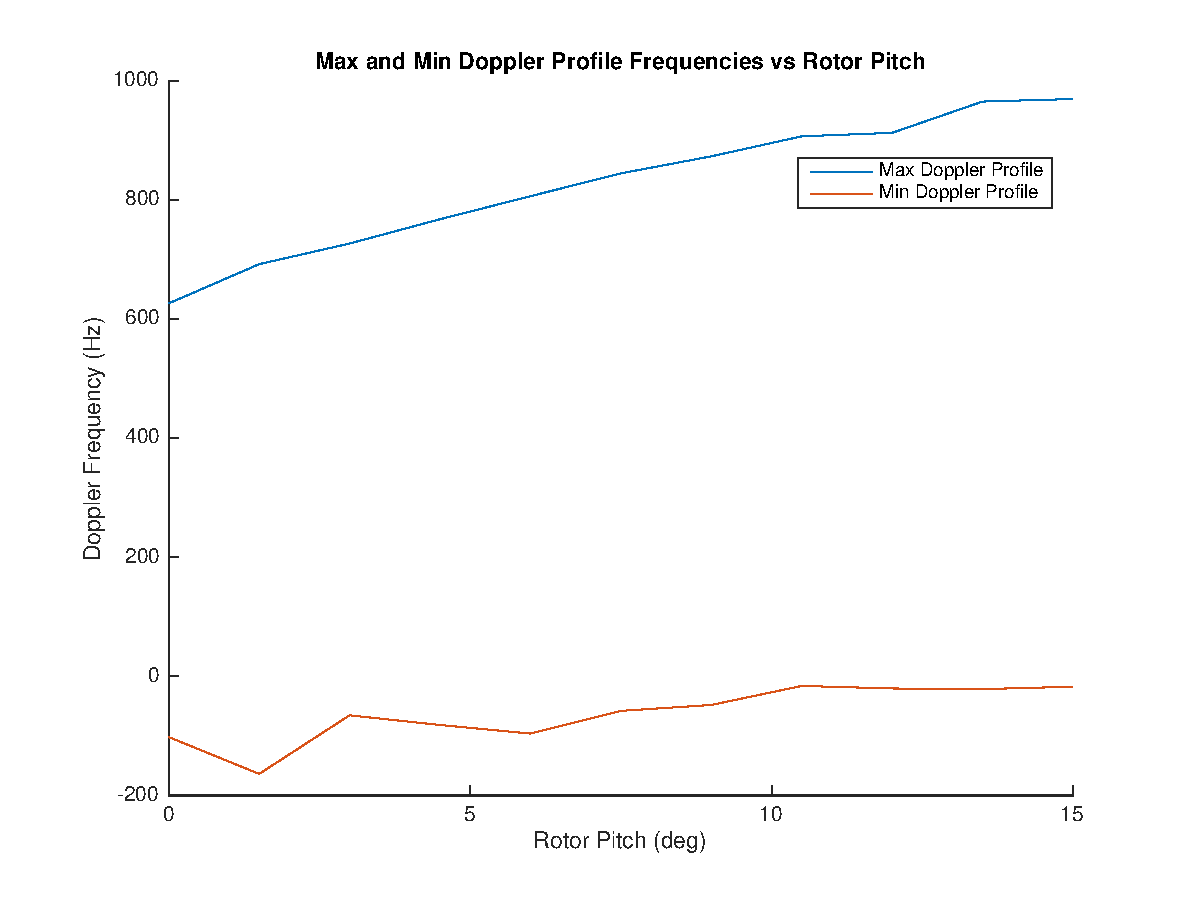
\includegraphics[width=10cm]{images/simulation/pitch_max_doppler.eps}
		\caption{Max and Min Envelope Frequencies vs Rotor Pitch with Tx Azimuth at 135\textdegree \space and Elevation at 54\textdegree}
		\label{fig:pitch_15_135deg}
	\end{center}
\end{figure}
%azimuth = 135deg, elevation = 54deg

From Figure \ref{fig:pitch_15_135deg} the effect of pitch on the maximum Doppler frequency is a linear increase between a pitch from 0\textdegree \space to 15\textdegree. Due to the linear increase, the pitch of the rotor blade can be accounted for when making measurements on subsequent simulation analysis. One issue does arise in when the transmitter is located underneath the helicopter which is shown in Figure \ref{fig:pitch_tx0}.

%figure of tx_0 and increasing pitch slope?
\begin{figure}
	\begin{center}
		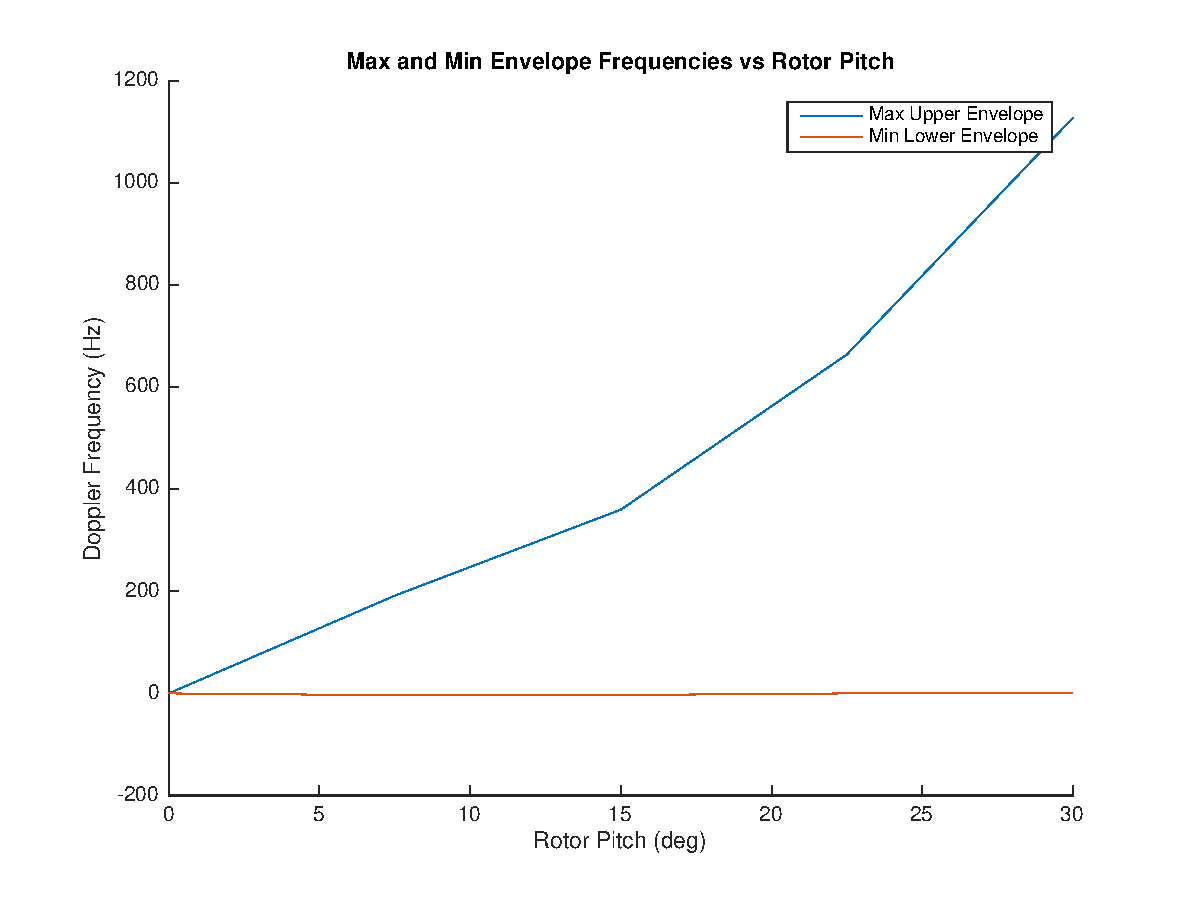
\includegraphics[width=10cm]{images/simulation/pitch_0txPos_max_doppler.eps}
		\caption{Max and Min Envelope Frequencies vs Rotor Pitch Transmitter Underneath the Helicopter}
		\label{fig:pitch_tx0}
	\end{center}
\end{figure}
%azimuth undefined, elevation 90deg

The pitch increases linearly at first then climbs at a much faster rate. This offset is caused by the pitch of the blade reflecting rays into the receiver which would be reflected back at the ground if the pitch was 0\textdegree. If the assumption is that the helicopter is hovering when these measurements take place, the pitch of the rotor will be much less than the maximum pitch available. This assumption will adjust the maximum pitch to 15\textdegree \space which will allow for the linear assumption to be fulfilled even when the transmitter is directly underneath the helicopter.

%figure max doppler vs range of 15 and 7.5 pitch and 0 pitch side by side
\begin{figure}
	\begin{center}
		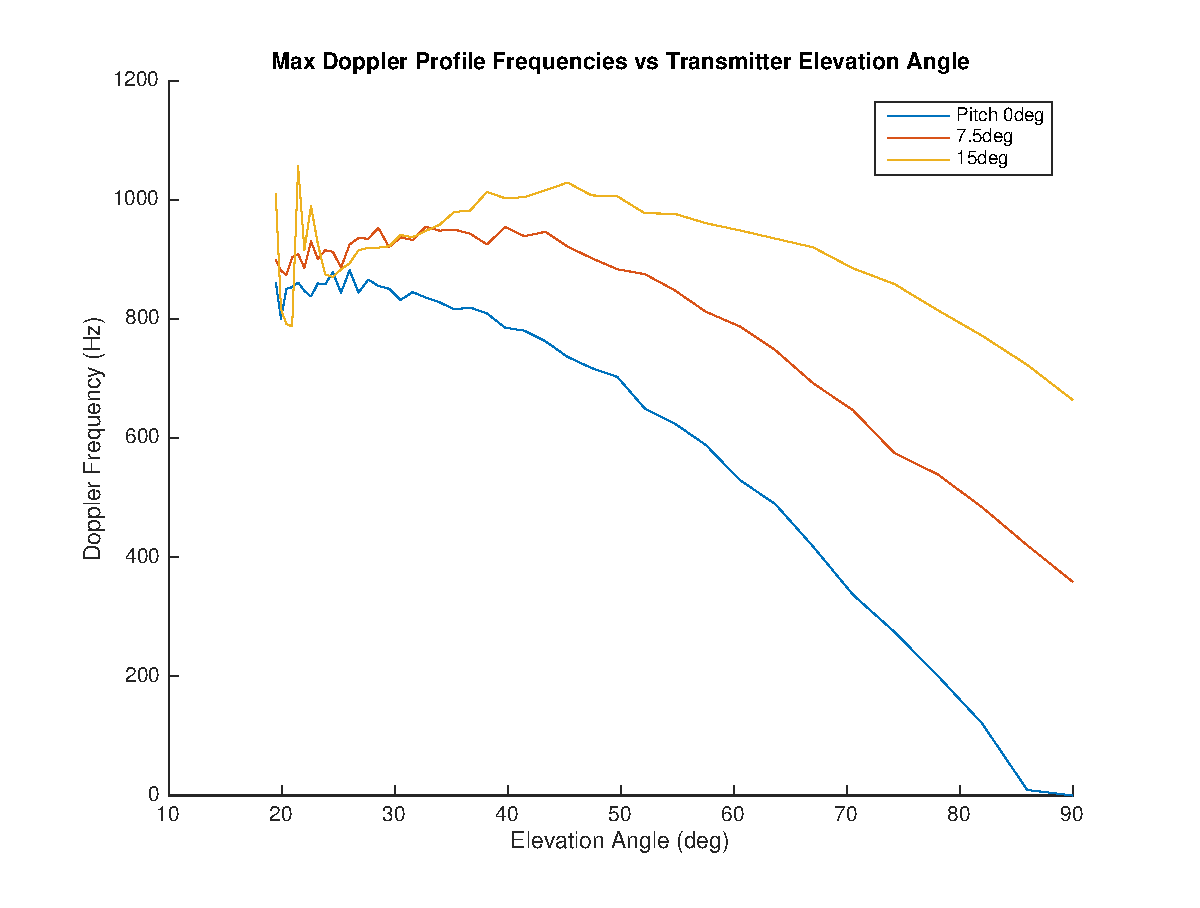
\includegraphics[width=10cm]{images/simulation/elevation_angle_with_pitch_max_doppler.eps}
		\caption{Max Envelope Frequencies vs Transmitter Elevation Angle}
		\label{fig:pitch_tx_elevation_angle}
	\end{center}
\end{figure}
%azimuth = 135deg

In Figure \ref{fig:pitch_tx_elevation_angle} the maximum Doppler versus elevation angles are initially shifted up in frequency from a pitch of 0\textdegree \space and, consequently, have changed in slope. This is because the rays hitting the blades from below are reflecting into the receiver at an angle that is closer to the direction of blade travel. The interesting thing about this plot is that the pitch envelopes actually become closer to the 0\textdegree \space envelope as the elevation angle becomes smaller. Figure \ref{fig:pitch_tx_elevation_angle_difference} shows the difference plotted over elevation angle.

\begin{figure}
	\begin{center}
		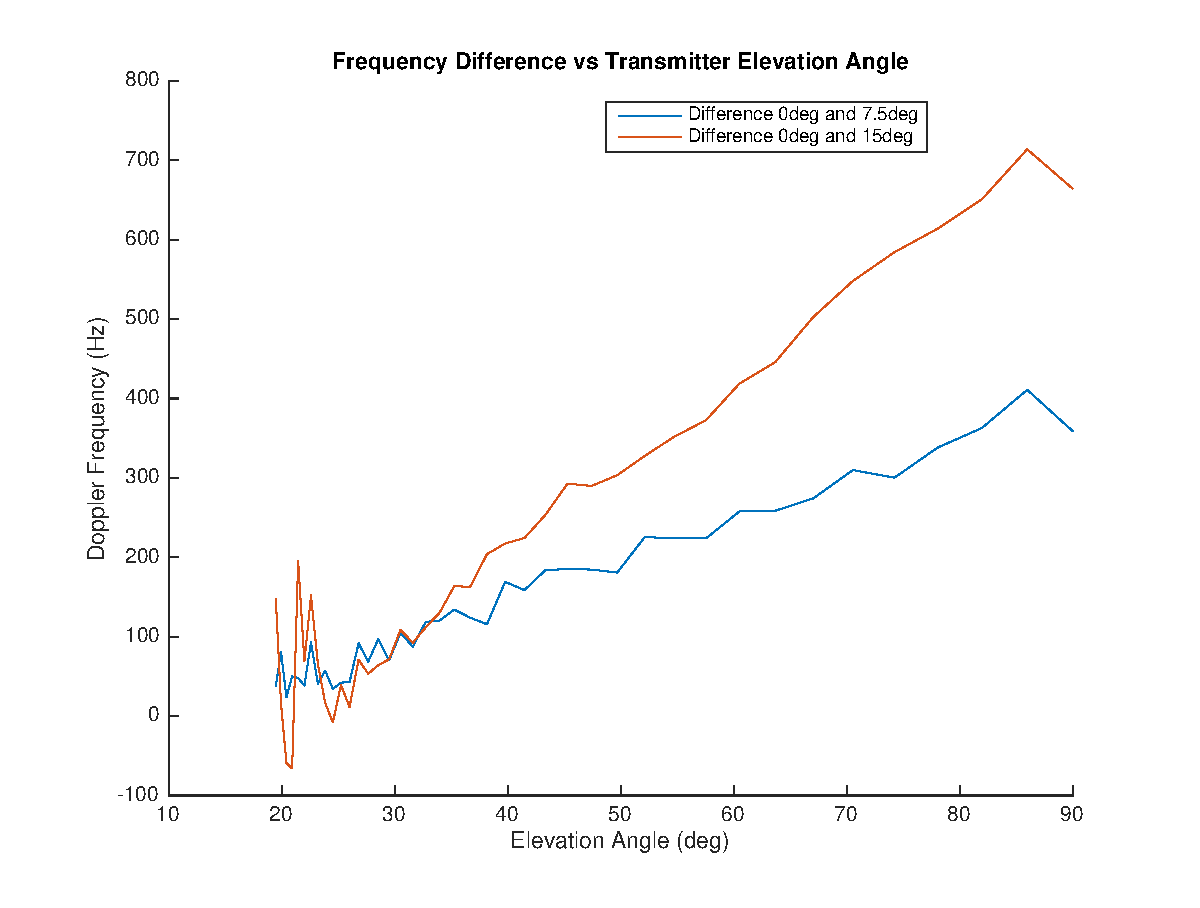
\includegraphics[width=10cm]{images/simulation/elevation_angle_with_pitch_max_doppler_Difference.eps}
		\caption{Frequency Difference vs Transmitter Elevation Angle}
		\label{fig:pitch_tx_elevation_angle_difference}
	\end{center}
\end{figure}

From Figure \ref{fig:pitch_tx_elevation_angle_difference} we can see that the difference in frequency changes linearly as the elevation angle decreases, the slope of which is based on the pitch angle. This slope would have to be characterized on the physical craft and can be accounted for due to its predictable nature.

%-----------------------------------------------------------------------------------------------------------------------------------------------------------------------
\section{Transmitter Azimuth Angle} \label{taa}
%display azimuth angle with respect to max doppler readings and describe patterns
The transmitter azimuth angle corresponds to the cardinal direction of the transmitter with respect to the front of the helicopter.

%figure of azimuth angle positions
\begin{figure}
	\begin{center}
		\includegraphics[width=9cm]{images/simulation/azimuth.eps}
		\caption{Transmitter Azimuth Angle Relationship}
		\label{fig:tx_azimuth_rel}
	\end{center}
\end{figure}

Where $\theta_{Az}$ is the azimuth angle. The azimuth angle of the transmitter in the simulation will effect the amount of Doppler added to the signal. This is due to the direction of the rotor blade rotation as it approaches both the receiver and the transmitter and how the rays reflect off the blade as it moves. From the model we see the amount of Doppler form a sinusoidal pattern as the azimuth angle goes from 0\textdegree \space to 360\textdegree. This is mirrored in the simulation shown in Figure \ref{fig:tx_azimuth_angle_200}.

%figure of doppler vs azimuth angle
\begin{figure}
	\begin{center}
		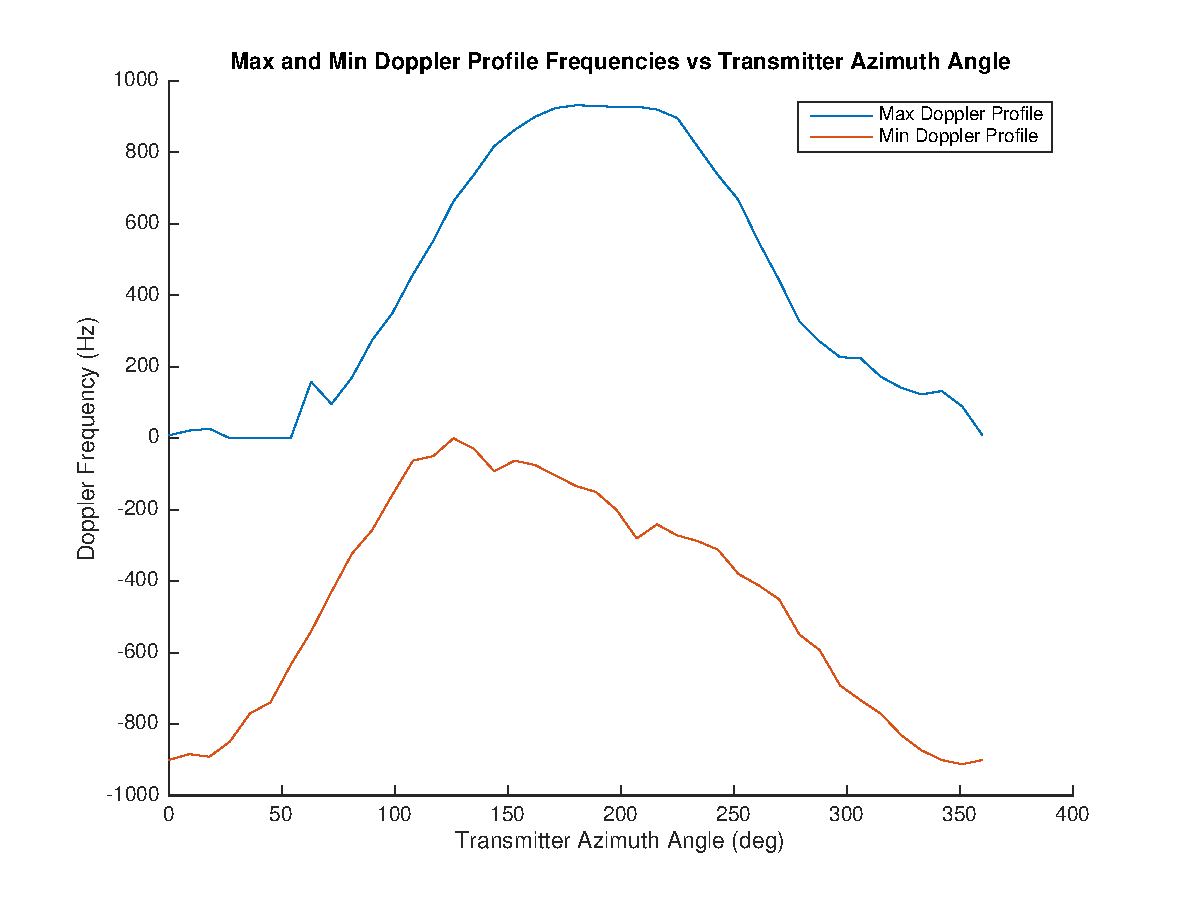
\includegraphics[width=10cm]{images/simulation/Azimuth_angle_200_max_doppler.eps}
		\caption{Max and Min Doppler Profile Frequencies vs Transmitter Azimuth Angle with Tx Elevation at 45\textdegree}
		\label{fig:tx_azimuth_angle_200}
	\end{center}
\end{figure}
%azimuth variable, elevation = 45deg

The graph in Figure \ref{fig:tx_azimuth_angle_200} shows both the maximum and the minimum measured Doppler as the azimuth angle completes a full rotation. The Doppler frequency follows the azimuth angle in a sinusoidal fashion. The sinusoidal pattern is held as the elevation angle changes shown in Figures \ref{fig:tx_azimuth_angle_50} and \ref{fig:tx_azimuth_angle_400}.

%figure of doppler and azimuth angle for different elevation angles.
\begin{figure}
	\begin{center}
		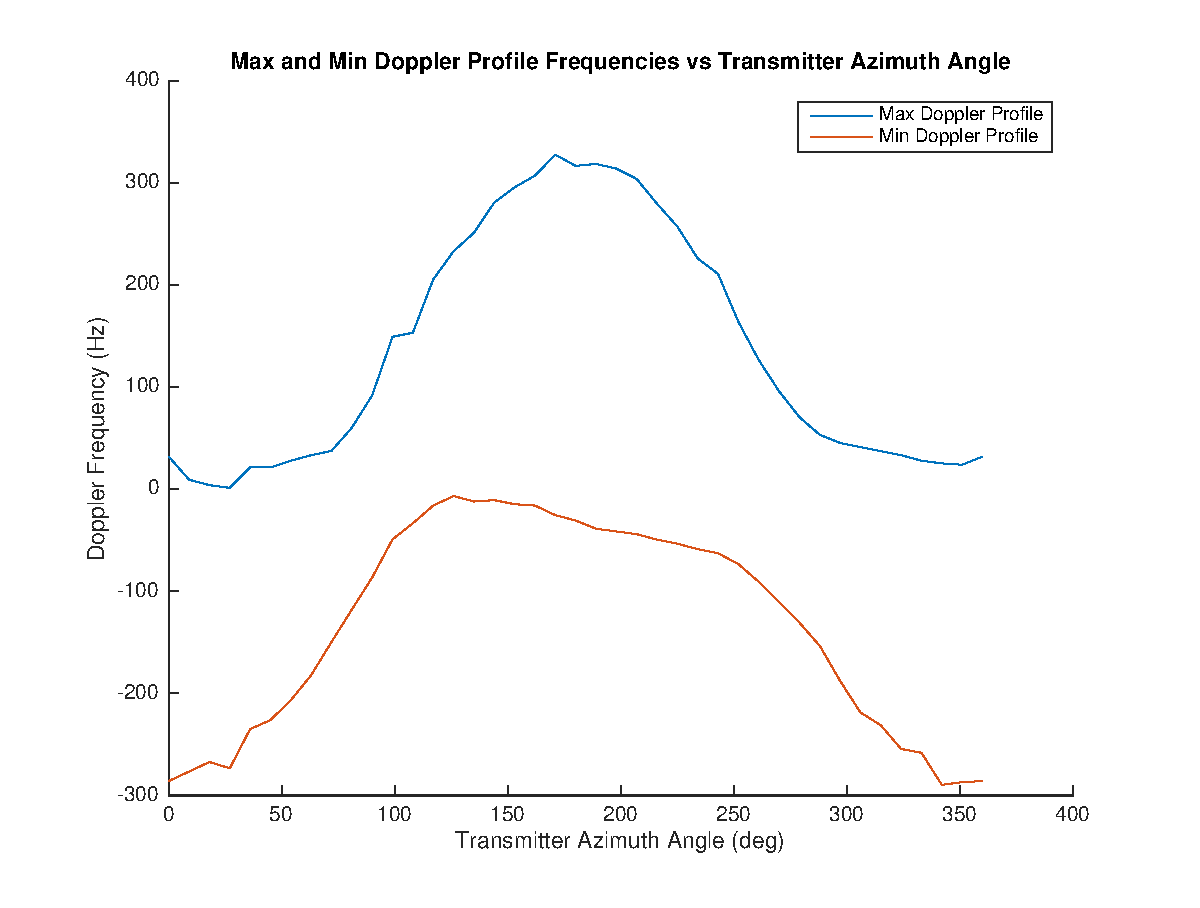
\includegraphics[width=10cm]{images/simulation/Azimuth_angle_50_max_doppler.eps}
		\caption{Max and Min Doppler Profile Frequencies vs Transmitter Azimuth Angle with Tx Elevation at 76\textdegree}
		\label{fig:tx_azimuth_angle_50}
	\end{center}
\end{figure}
%azimuth variable, elevation = 76deg

\begin{figure}
	\begin{center}
		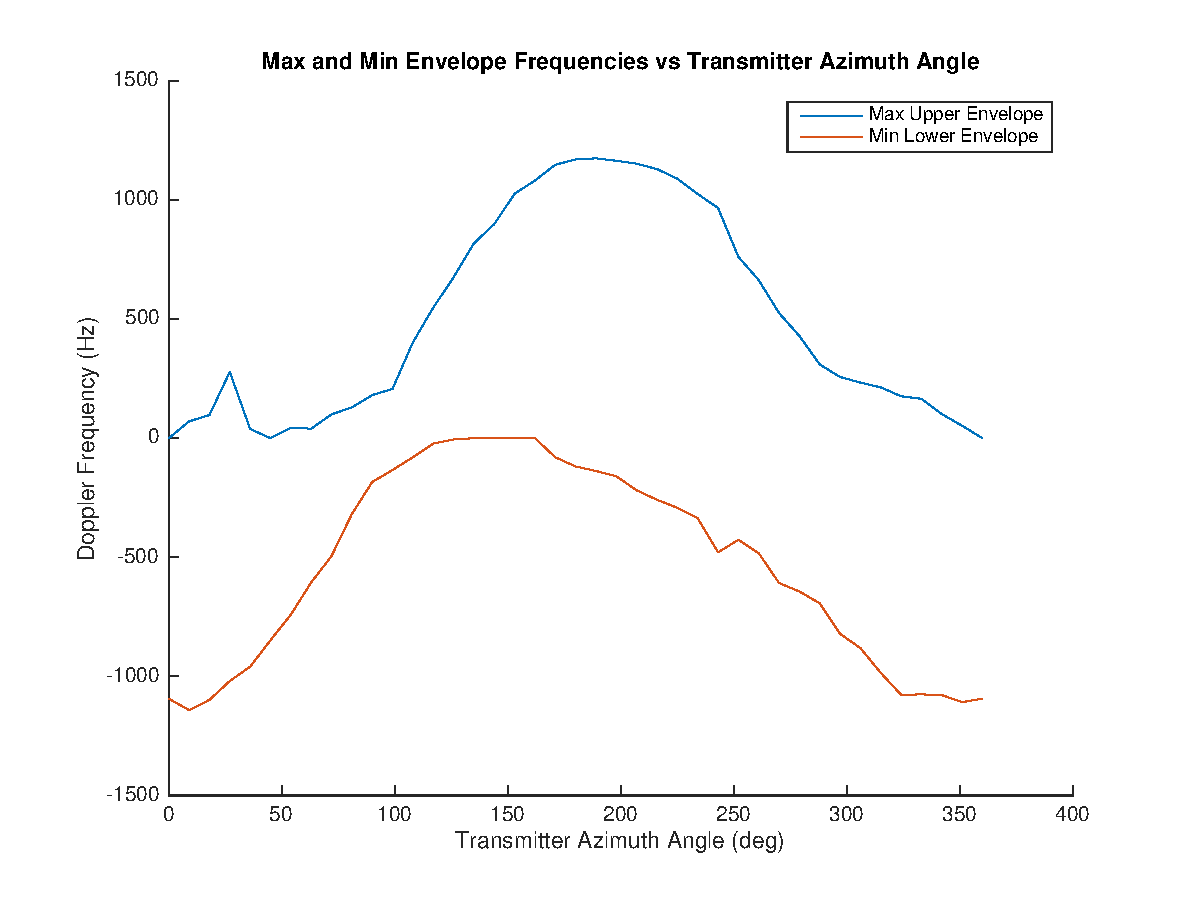
\includegraphics[width=10cm]{images/simulation/Azimuth_angle_400_max_doppler.eps}
		\caption{Max and Min Doppler Profile Frequencies vs Transmitter Azimuth Angle with Tx Elevation at 26.5\textdegree}
		\label{fig:tx_azimuth_angle_400}
	\end{center}
\end{figure}
%azimuth variable, elevation = 26.5deg

%description
The sinusoidal pattern of minimum and maximum Doppler frequencies are only present when the receiver is located away from the axis of rotation. This is shown in Figure \ref{fig:tx_azimuth_rx0} which is devoid of any sinusoidal pattern and remains constant as the transmitter azimuth angle is changed. 

%figure of 0 rx position
\begin{figure}
	\begin{center}
		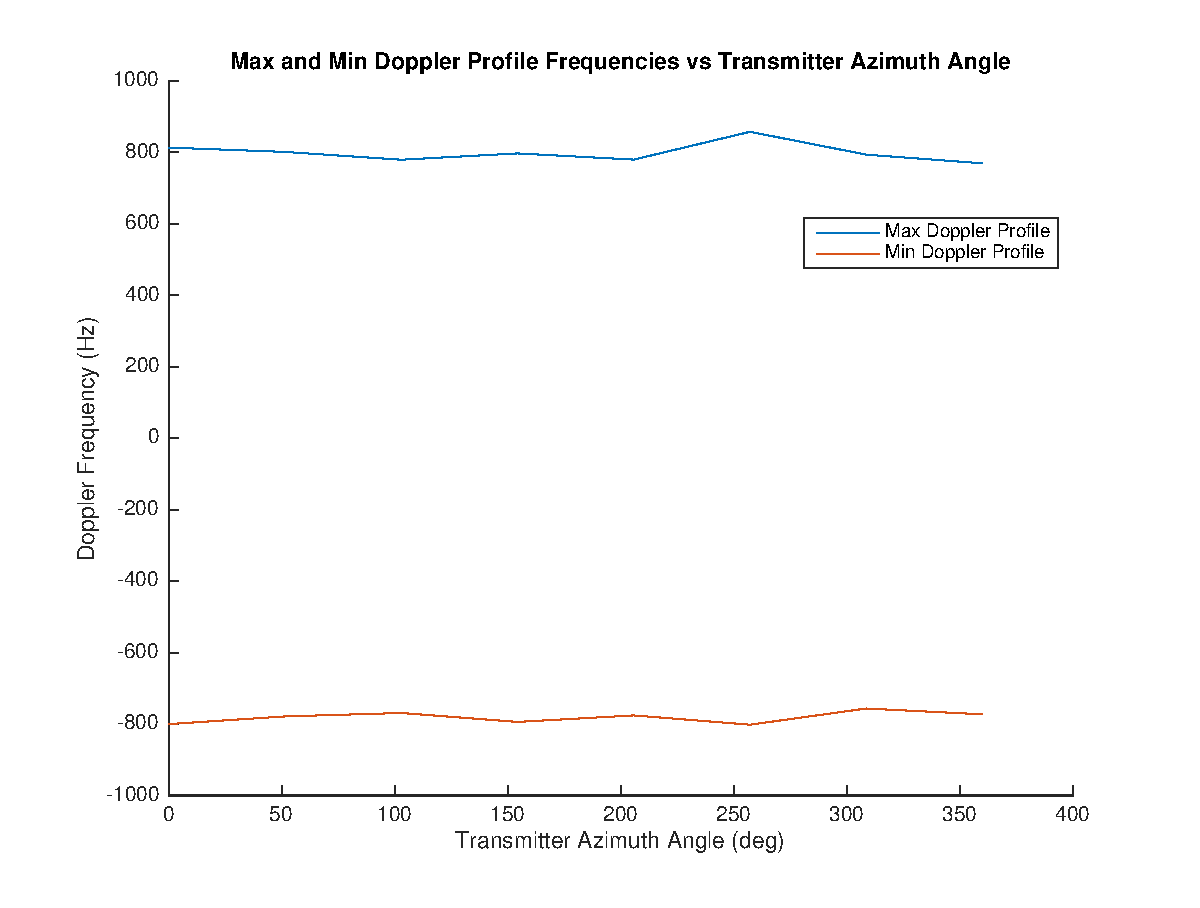
\includegraphics[width=10cm]{images/simulation/Azimuth_angle_rx0_max_doppler.eps}
		\caption{Max and Min Envelope Frequencies vs Transmitter Azimuth Angle with Rx at Axis of Rotation}
		\label{fig:tx_azimuth_rx0}
	\end{center}
\end{figure}

Therefore all future simulations will set the receiver near the tip of the rotor which would simulate the receiver being in the nose of the helicopter.

Pitching the blade modifies the results of the azimuth sweep when compared to Figure \ref{fig:tx_azimuth_angle_200}. The resulting minimum and maximum envelope frequencies versus azimuth angle for pitch are shown in Figure \ref{fig:pitch_azimuth_rev}. This occurs because the pitch of the blade angles RF reflections differently according to transmitter azimuth. When the transmitter is located between 90\textdegree \space and 270\textdegree \space pitch causes an increase in Doppler but elsewhere it decreases the amount of Doppler shift. The decrease is caused by the blade surface top reflecting receding Doppler away from the receiver at those angles.

%azimuth pitch effect
\begin{figure}
	\begin{center}
		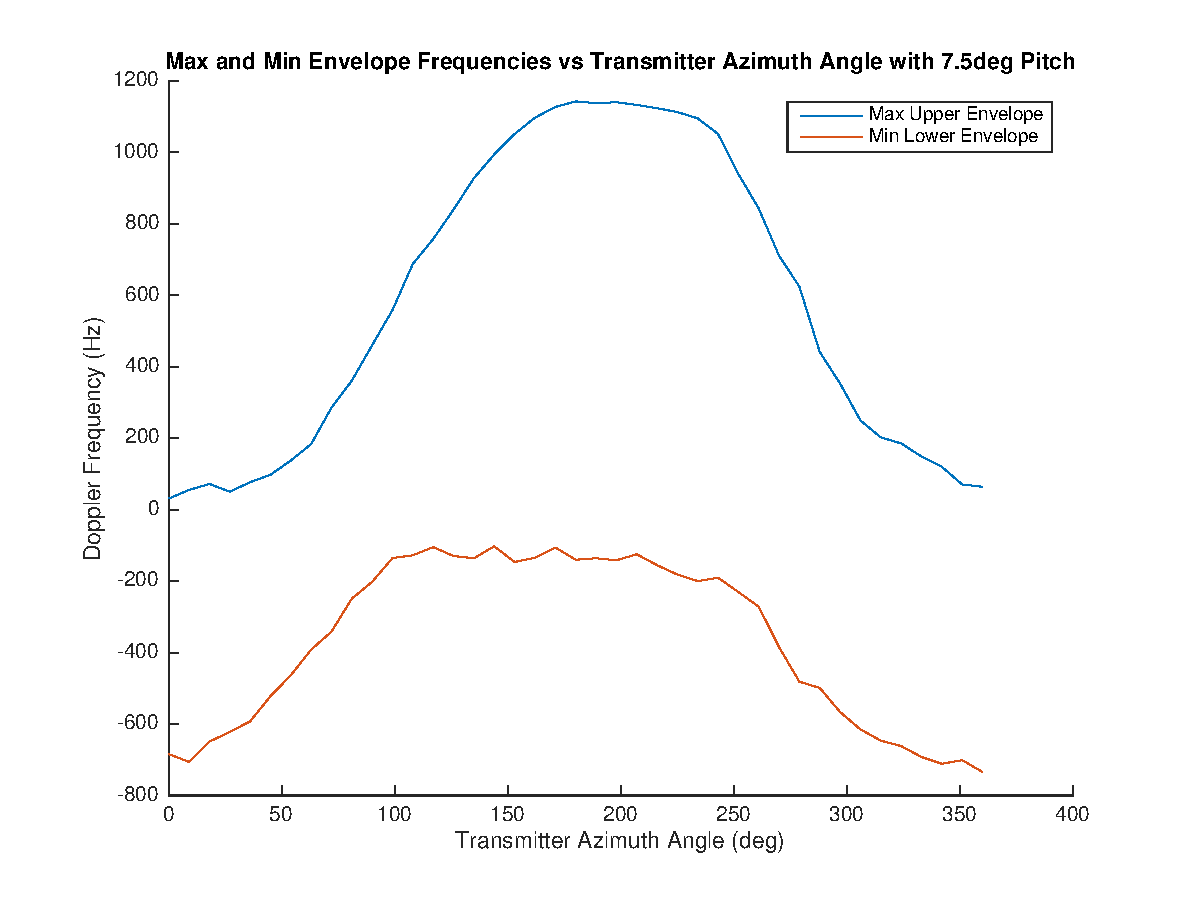
\includegraphics[width=10cm]{images/simulation/pitch_azimuth_rev.eps}
		\caption{Max and Min Envelope Frequencies vs Transmitter Elevation Angle with 7.5deg Pitch}
		\label{fig:pitch_azimuth_rev}
	\end{center}
\end{figure}

The effect of the azimuth angle on the maximum measured Doppler is characterized in section \ref{sec:transmitter_azimuth_angle_estimation}

%-----------------------------------------------------------------------------------------------------------------------------------------------------------------------
\section{Transmitter Elevation Angle} \label{sec:tea}
%display elevation angle with respect to max doppler readings and describe patterns
The transmitter elevation angle is the angle between the helicopter rotor and the position of the transmitter shown in Figure \ref{fig:azimuth_rel} where $\theta_{El}$ is the elevation angle. 

%figure of position of elevation angle with respect to rotor
\begin{figure}
	\begin{center}
		\includegraphics[width=10cm]{images/simulation/elevation.eps}
		\caption{Transmitter Elevation Angle}
		\label{fig:azimuth_rel}
	\end{center}
\end{figure}

The smaller elevation angles mean that the transmitter is farther away from the helicopter. The elevation angle in relation to the distance of the transmitter is shown by Figure \ref{fig:tx_range_elevation_rel}.

%figure of range vs elevation angle.
 \begin{figure}
	\begin{center}
		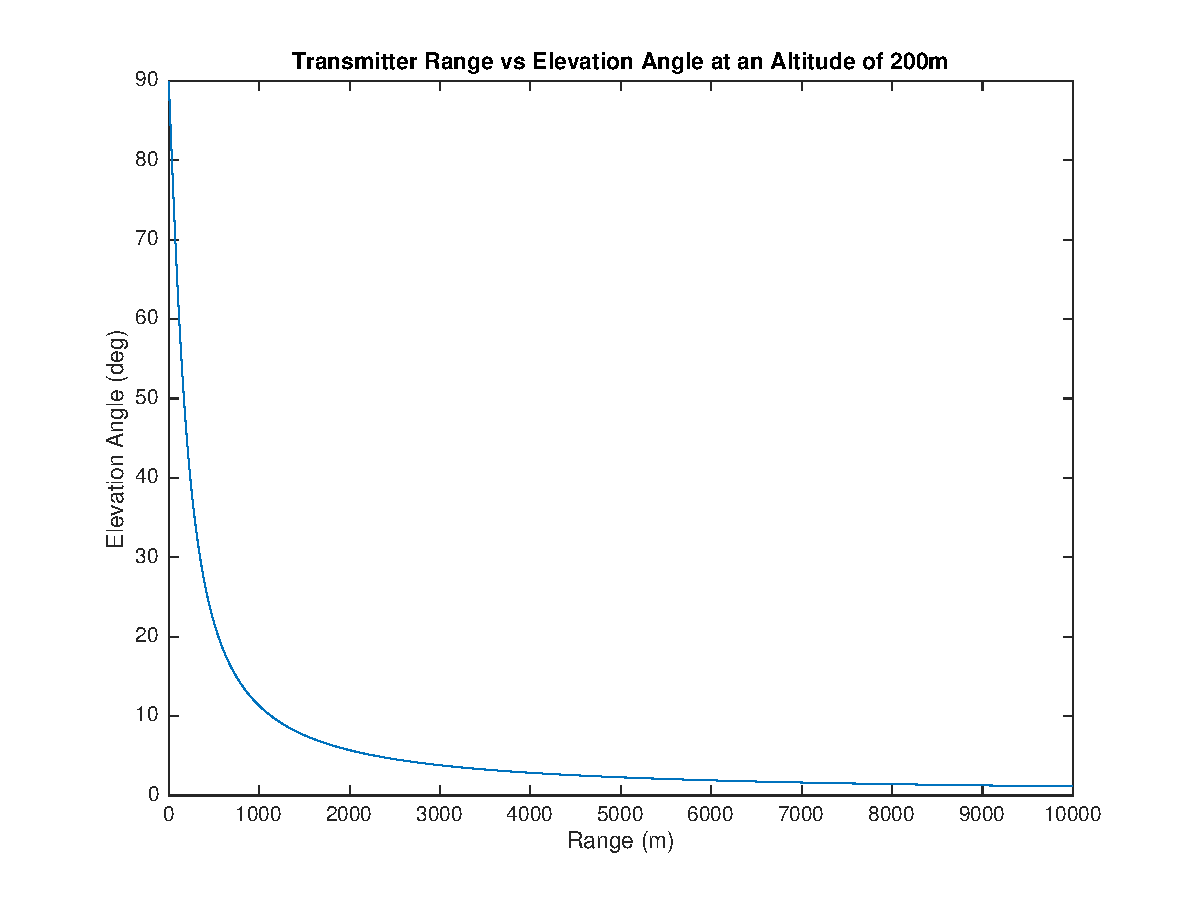
\includegraphics[width=10cm]{images/simulation/range_elevation_rel.eps}
		\caption{Transmitter Range vs Elevation Angle at an Altitude of 200m}
		\label{fig:tx_range_elevation_rel}
	\end{center}
\end{figure}

The elevation angle of the transmitter in the simulation will effect the amount of Doppler added to the signal. This is due to the rays having a vector component in the direction of the travel of the rotor. When the transmitter is directly underneath the rotor and receiver, there is no vector component in the direction of rotor travel so the reflected signal is not Doppler shifted. From the model we see the amount of Doppler increase as the elevation angle decreases. This is mirrored in the simulation shown in Figure \ref{fig:tx_elevation_135deg} where the maximum measured Doppler as the elevation angle increases.

%figure of doppler vs (elevation angle)
 \begin{figure}
	\begin{center}
		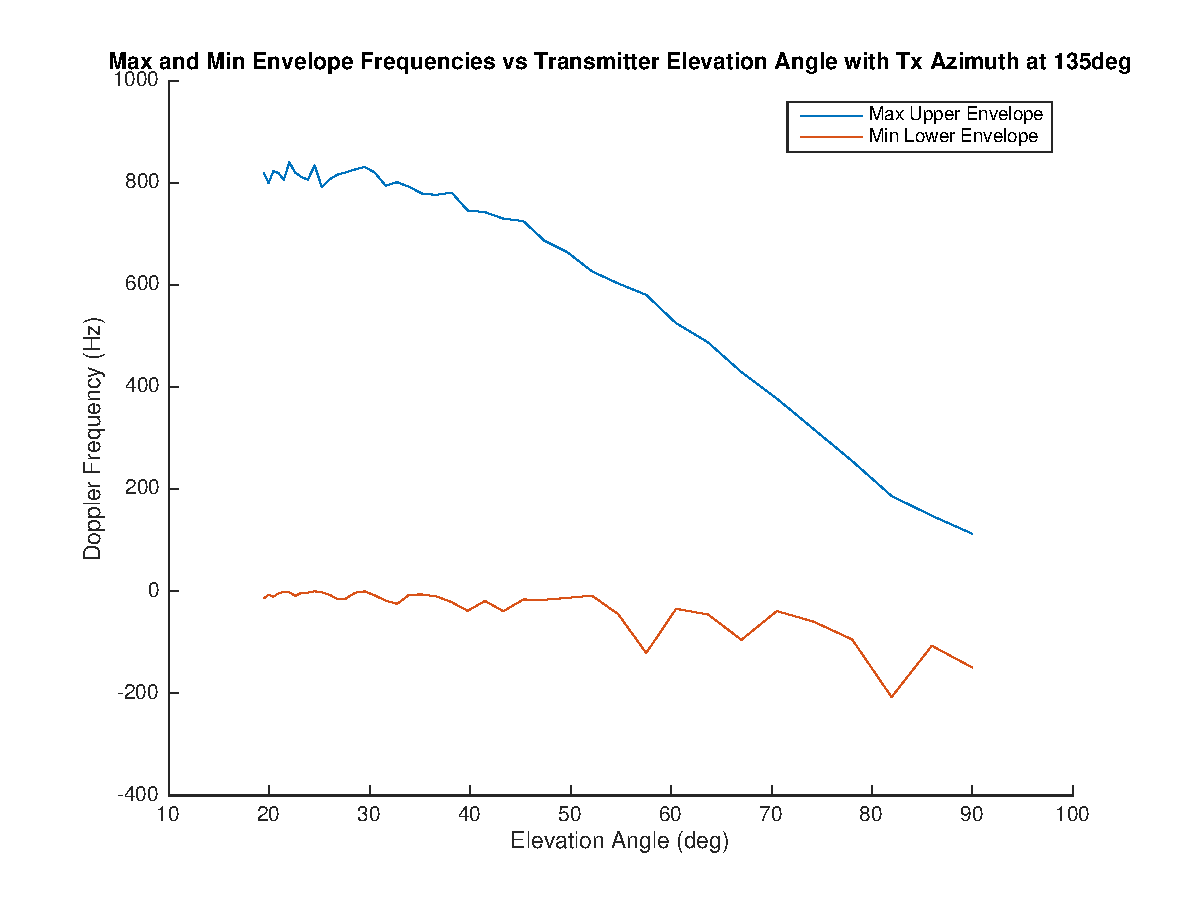
\includegraphics[width=10cm]{images/simulation/elevation_angle_max_doppler_135deg.eps}
		\caption{Max and Min Envelope Frequencies vs Transmitter Elevation Angle with Tx Azimuth of 135deg}
		\label{fig:tx_elevation_135deg}
	\end{center}
\end{figure}
%azimuth = 135deg, elevation = var

Looking back at the geometric models for transmitter azimuth angles of 0\textdegree \space \ref{fig:3D_model_0az_doppler}, 90\textdegree \space \ref{fig:3D_model_90az_doppler}, 180\textdegree \space \ref{fig:3D_model_180az_doppler}, and 270\textdegree \space \ref{fig:3D_model_270az_doppler} and their simulated counterparts shown in Figure \ref{fig:verify}. We see that the ray traced results match their projections on the maximum and minimum envelope Doppler as transmitter elevation angle changes. The Doppler values do not match exactly but the trends are very similar.

\begin{figure}
\centering
	\subfloat[0\textdegree]{
	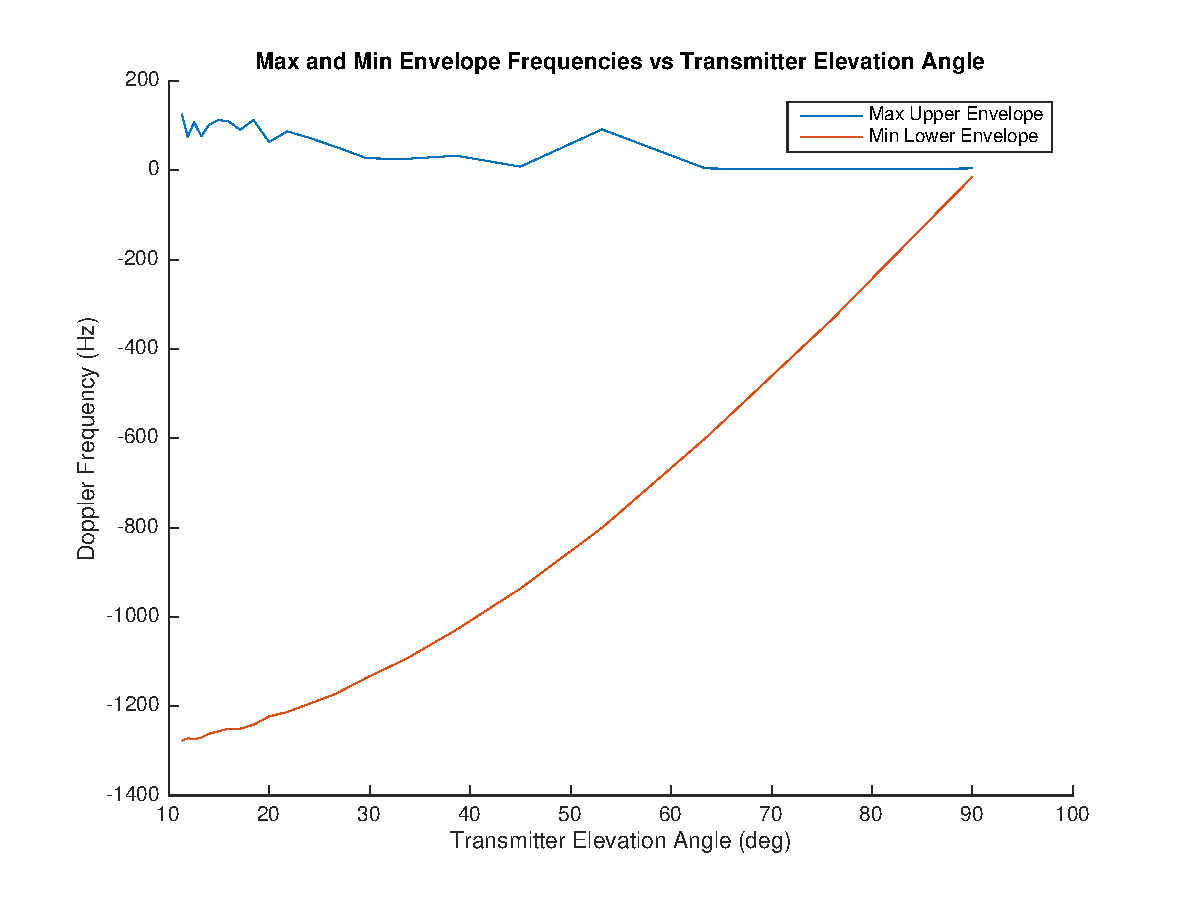
\includegraphics[width=7cm]{images/simulation/elevation_angle_max_doppler_0deg.eps}
	}
	\subfloat[90\textdegree]{
	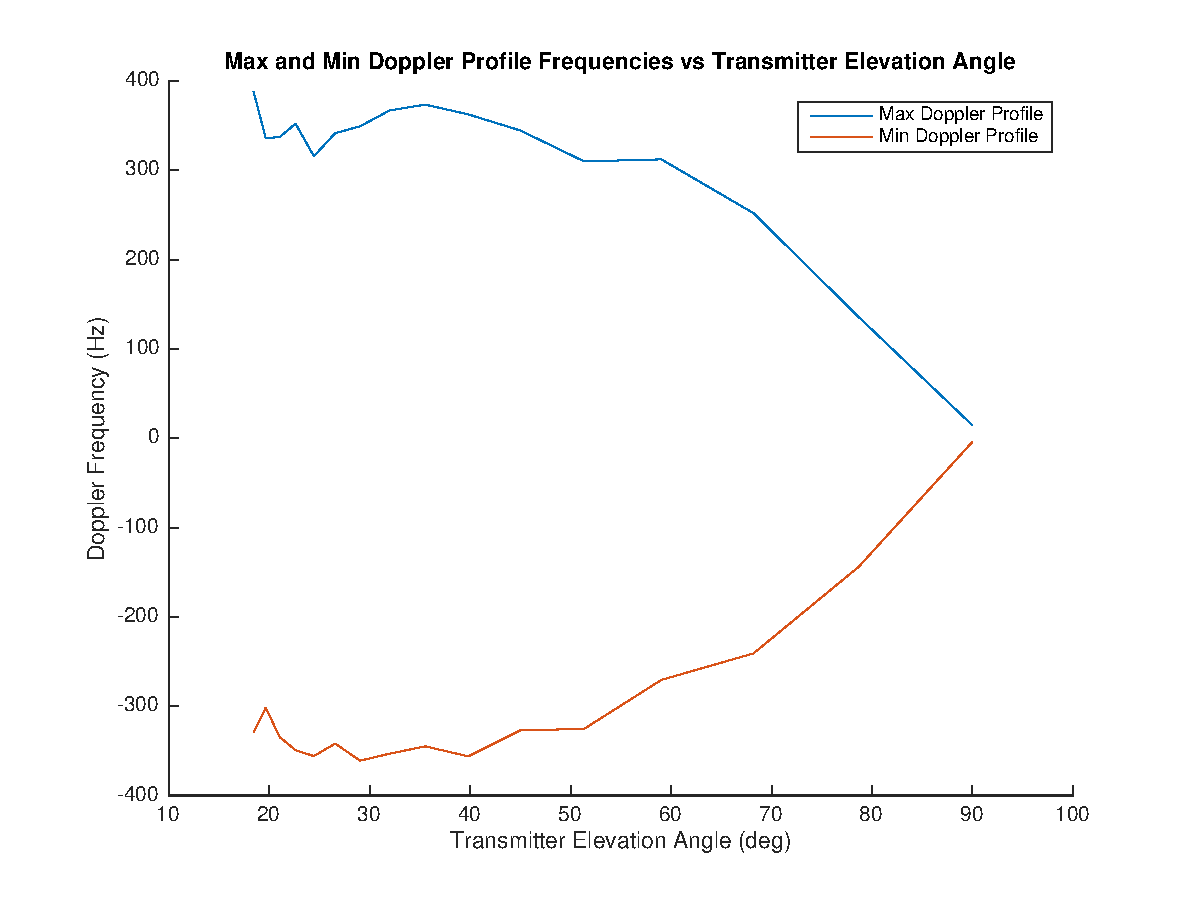
\includegraphics[width=7cm]{images/simulation/elevation_angle_max_doppler_90deg.eps}
	}
	\newline
	\subfloat[180\textdegree]{
	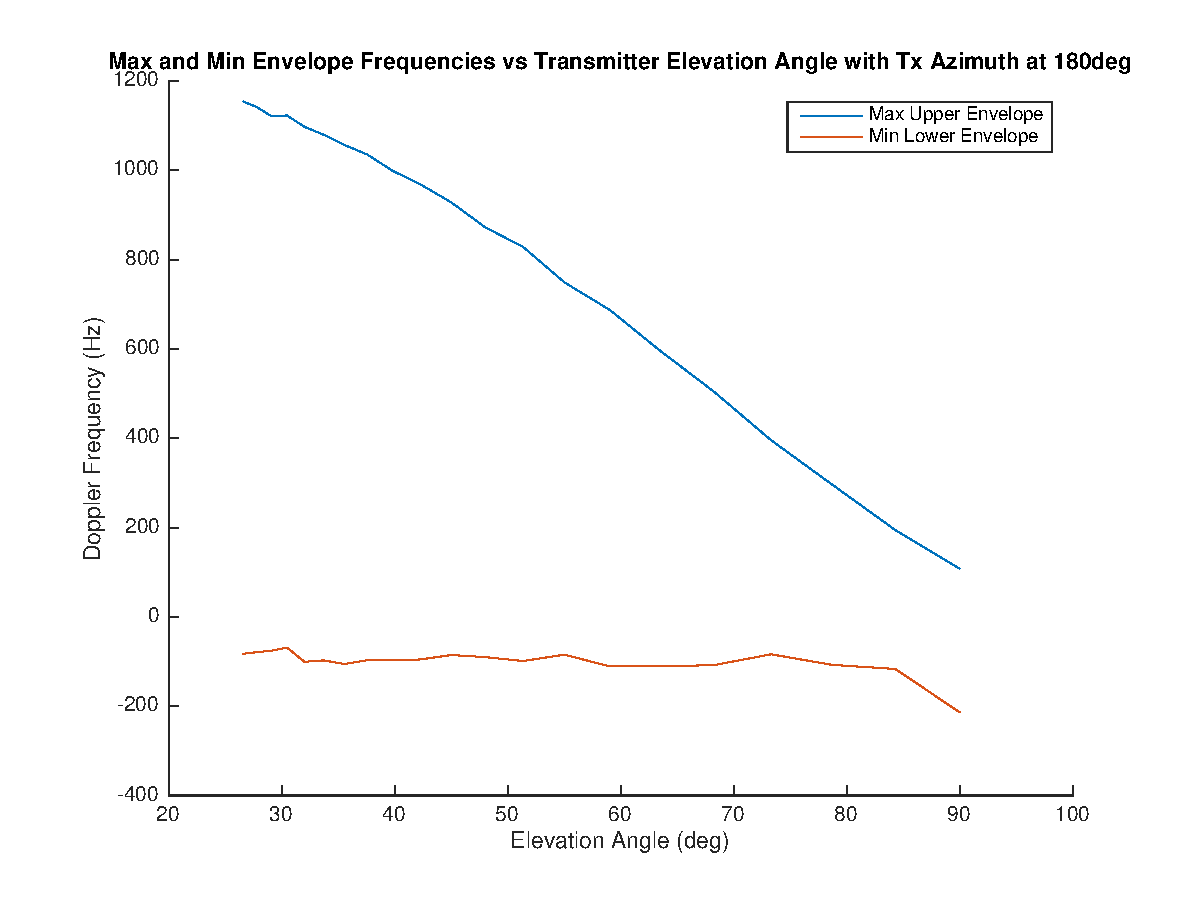
\includegraphics[width=7cm]{images/simulation/elevation_angle_max_doppler_180deg.eps}
	}
	\subfloat[270\textdegree]{
	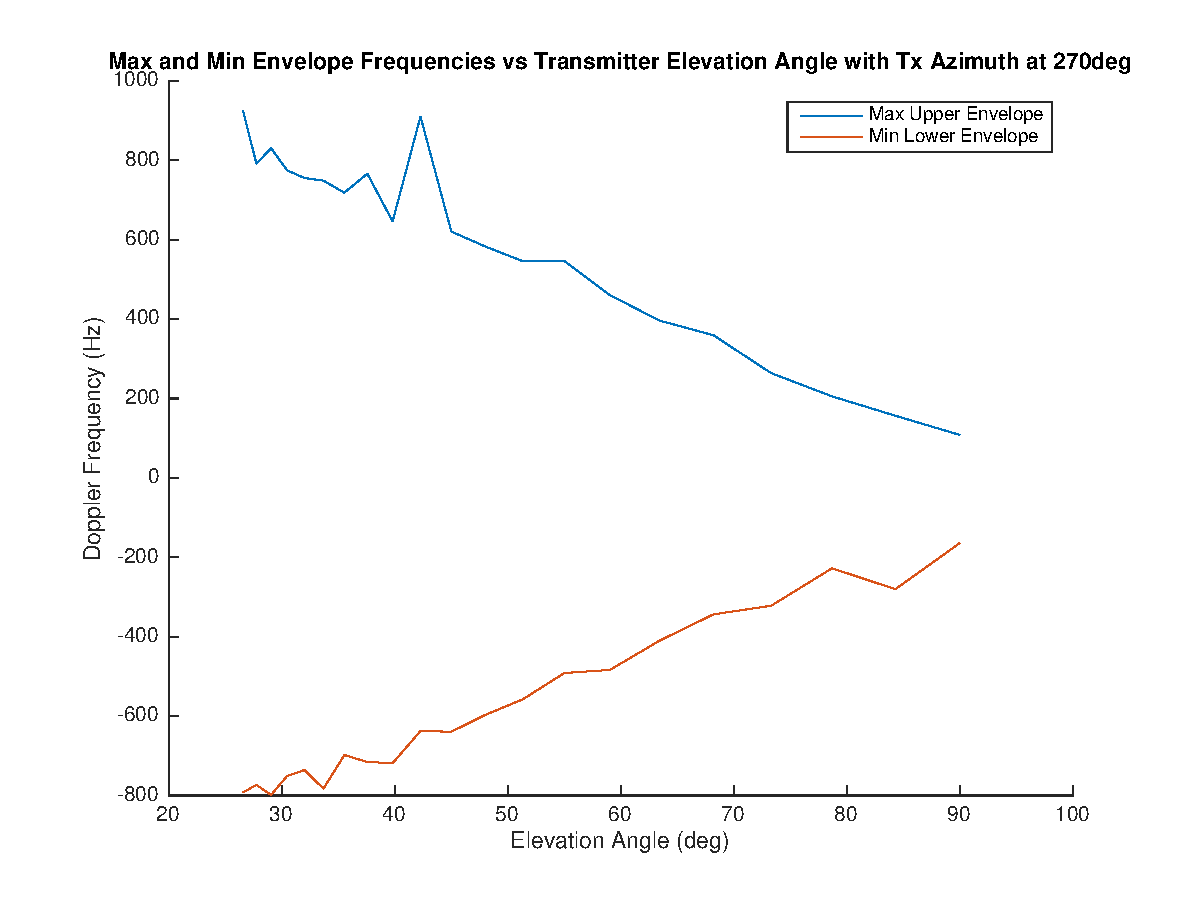
\includegraphics[width=7cm]{images/simulation/elevation_angle_max_doppler_270deg.eps}
	}
\caption{Doppler Profile vs. Transmitter Elevation angle for various Azimuth angles.}
\label{fig:verify}
\end{figure}

The effect of elevation angle on the maximum measured Doppler will be characterized in section \ref{sec:transmitter_elevation_angle_estimation}.



